\documentclass{article}
\usepackage{iclr2016_conference,times}

\usepackage{subfig}
\usepackage{float}
\usepackage{hyperref}
\usepackage{url}
\usepackage{amsmath,amssymb}
\usepackage{natbib}
\usepackage{wrapfig}
\usepackage{graphicx}
\bibliographystyle{abbrvnat}

\title{Project Proposal\vspace{-6pt}\\{\large Andrea F. Daniele $\hspace{2cm}$ Max X. Liu $\hspace{2cm}$ Noah A. Hirsch }}

\begin{document}

\maketitle


\vspace{-1.2cm}

\section*{Introduction}
\vspace{-.3cm}
As autonomous vehicles become more prevalent, a large concern is ensuring safety. 
An important consideration for safety is how autonomous vehicles communicate with each other. 
More specifically, we want to investigate the optimal number of vehicles for each vehicle to communicate with. 
Obviously, communicating with as many vehicles as possible would be ideal. 
The problem is that communicating with each vehicle takes time, and the time spent communicating 
with some distant car might be better spent keeping a nearer car more up to date. 
The goal of this project is to study what is the best number of vehicles a self-driving car should 
communicate with in order to maximize safety while minimizing the cost.

\section*{Problem}
\vspace{-.3cm}
In order to increase autonomous vehicle safety and optimize route planning, vehicles must be able to effectively communicate with one another. Specifically in hazardous situations, it is critical to communicate useful data to relevant vehicles.

\section*{Challenges}
\vspace{-.3cm}
One of the main challenges in fleet-level communication is the choice of a network infrastructure suitable
for the task. WiFi networks are fast and cheap to deploy but have a limited range. Communication via satellites
offer an unlimited range but it is expensive to deploy. Another challenge is that of deciding how many cars
to share information with and how many cars to get information from. Even though self-driving vehicles are
expected to be capable of processing a lot of information locally, we still need to minimize the impact of a 
fleet-level communication architecture on the on-board computer.

\section*{Proposed Approach and Timeline}
\vspace{-.3cm}
We will run our experiments on a fleet of real robots driving autonomously in a small town 
known as Duckietown~(Figure \ref{fig:duckietown}).

\begin{wrapfigure}{r}{0.5\textwidth}
    \centering
    \vspace{-12pt}
    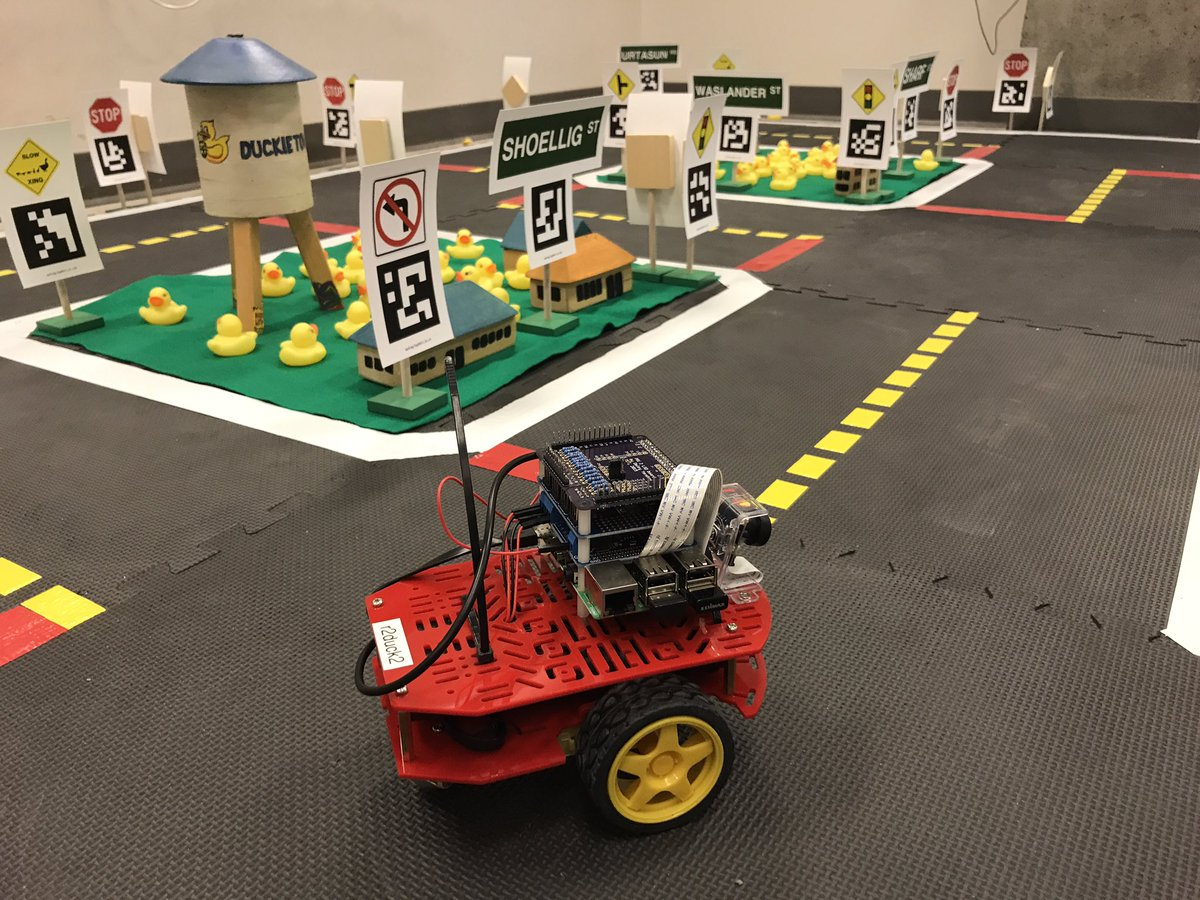
\includegraphics[width=0.48\textwidth]{figures/duckietown.jpg}
    \caption{Duckietown at TTIC \label{fig:duckietown}}
    \vspace{-6pt}
\end{wrapfigure}

In the first $2$ weeks, we will deploy a communication infrastructure on a fleet of about 8 robots.
These robots will be connected to a common WiFi network.
Due to the size of the town, all the robots would be able to physically communicate with each other.
We will simulate smaller communications ranges around each robot by artificially dropping packets after a 
certain distance.
In the last $4$ weeks we will run experiments in which, at a certain time instant, one of the robots will perceive
the presence of an hazardous situation and communicate it to the closest $N$ robots via an emergency message
with the location of the event. Once a robot receives an emergency message, it will immediately stop if the 
event being notified is located along its current path to its goal. In these experiments,
we will measure the performance of the communication protocol as the reaction time of the robots stopping 
upon receiving an emergency message.

\end{document}
